\documentclass[a4paper,12pt]{article}

\usepackage{amsmath,amssymb,multicol,tikz,enumitem}
\usepackage[margin=2cm]{geometry}
%\usetikzlibrary{calc}
\usepackage{amsmath}
\usepackage{amsthm}
\usepackage{thmtools}
\usepackage{hyperref}
\usepackage{enumerate}
\usepackage{xcolor}
\usepackage{fancyvrb}

\pagestyle{empty}

\newcommand\Q{\mathbf{Q}}
\newcommand\R{\mathbf{R}}
\newcommand\Z{\mathbf{Z}}

\usepackage{array}
\newcolumntype{P}[1]{>{\centering\arraybackslash}p{#1}}

\newcommand\indd{${}$\hspace{20pt}}

\declaretheoremstyle[headfont=\normalfont\bfseries,notefont=\mdseries\bfseries,bodyfont = \normalfont,headpunct={:}]{normalhead}
\declaretheorem[name={Uzdevums}, style=normalhead,numberwithin=section]{problem}

\setcounter{section}{108}

\setlength\parindent{0pt}

\begin{document}

\clearpage
\begin{center}
\parbox{3.5cm}{\flushleft\bf Skaitļu teorija \newline ATV} \hfill {\bf\LARGE Uzdevumu lapa \#8} \hfill \parbox{3.5cm}{\flushright\bf 2021-02-24} %\\[2pt]
\end{center}

%\hrule\vspace{2pt}\hrule
\hrule


%\vspace{20pt}
%2016.gada Valsts olimpiādes 3.kārtas 2.posma uzdevumi.

\vspace{10pt}
\begin{problem}
Atrast visas funkcijas $f$, kas definētas reālo skaitļu kopā, pieņem reālas vērtības un visiem reāliem skaitļiem $x,y$
apmierina vienādību
\[ f(x - f(x - y)) = f(x + y) - x. \]
\end{problem}

\vspace{10pt}
\begin{problem}
%8.2. 
Kvadrātu, kura izmēri ir $9 \times 9$ rūtiņas, sagrieza tā, ka katra no iegūtajām daļām bija vai nu 1.att., vai 2.att., vai
3.att. redzamā figūra. Kāds ir mazākais skaits 3.att. redzamo figūru, ko varēja iegūt?

%\begin{figure}[!htb]
\center{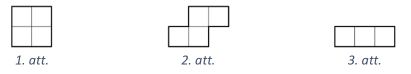
\includegraphics[width=3.5in]{atv-08/poliminoes.png}}
%\caption{\label{fig:poliminoes} Polimino images.}
%\end{figure}
\end{problem}


\vspace{10pt}
\begin{problem}
Atrast visus tādus pirmskaitļus $p$, ka $3^{p^2 - 1} + 20$ arī ir pirmskaitlis!
\end{problem}



\vspace{10pt}
\begin{problem}
Trijstūrī $ABC$ novilkta mediāna $CM$. Riņķa līnija ar diametru $CM$ krusto nogriežņus $AC$ un $BC$ attiecīgi punktos $P$ un $Q$. 
Zināms, ka $AB  \parallel PQ$ un $\sphericalangle CAB = \alpha$. 
Kādas ir $\sphericalangle ACB$ iespējamās vērtības?

\end{problem}



\vspace{10pt}
\begin{problem}
Vai eksistē tāda bezgalīga naturālu skaitļu virkne $(a_n)$, ka katram naturālam $n$, 
skaitļu $a_{n+1},a_{n+2}, \ldots, a_{n+a_n}$ vidējais
aritmētiskais ir vienāds ar $n$?
\end{problem}




\end{document}

